%\begin{figure}[p]
%    \centering
%    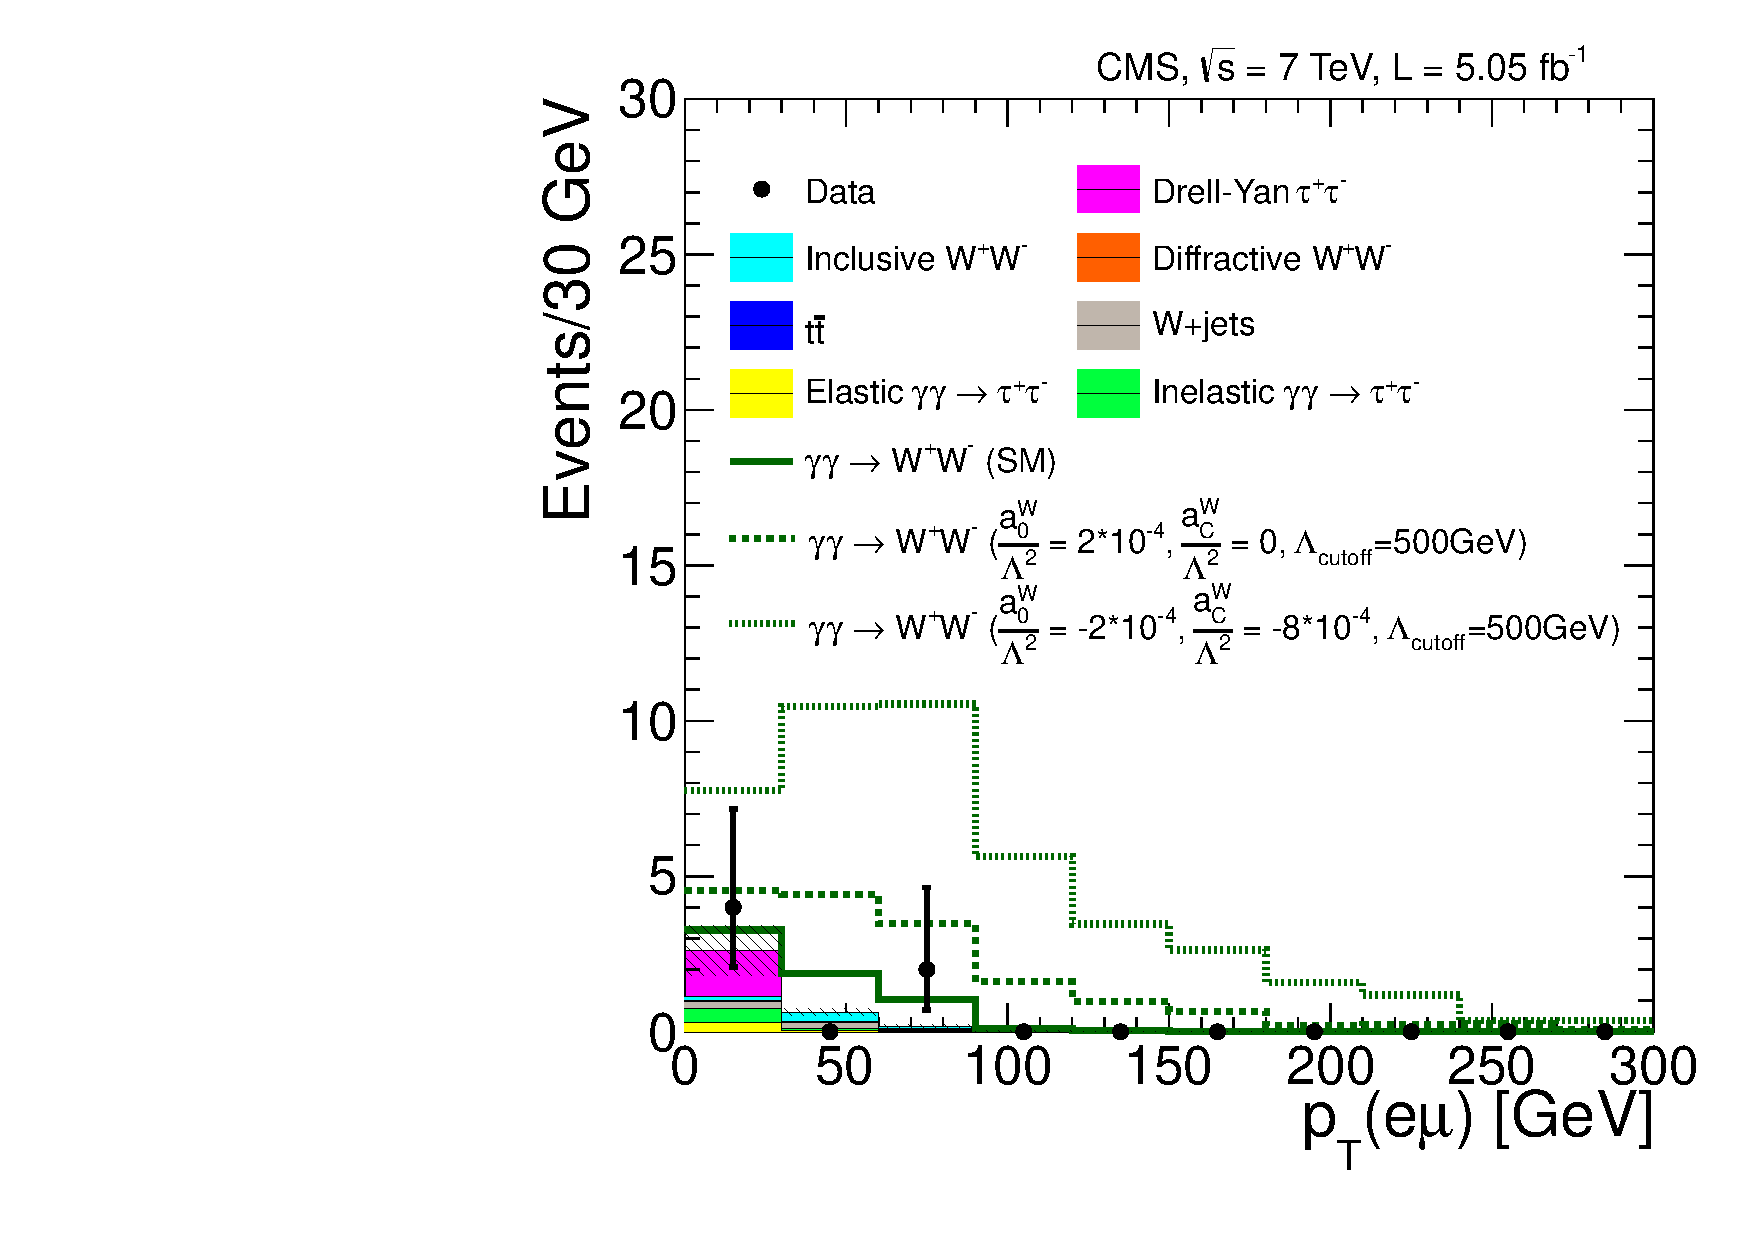
\includegraphics[height=0.3\textheight]{figures/ss-exclboson-ww-cms7tev}
%    \caption{}
%    \label{fig:ss-exclboson-ww-cms7tev}
%\end{figure}
%CMS WWexcl 7 \TeV~\cite{Chatrchyan:2013foa}

In addition to exclusive single boson production, CMS and ATLAS have
evidence for exclusive diboson production, in two different channels.
In one of them, CMS~\cite{Khachatryan:2016mud} has performed a search
for exclusive diboson production via protons emitting (possibly
quasi-) real photons which rescatter to produce $W^+W^-$ pairs:
$pp \to p^{(*)}W^+ W^- p^{(*)} \to p^{(*)}\mu^{\pm}e^{\mp}p^{(*)}$,
where $p^*$ admits the possibility that the protons dissociate into an
undetected system.  Such production is characterized by a
$\mu^{\pm}e^{\mp}$ pair which has no underlying event activity typical
of proton-proton hard scattering.  By selecting a $\mu^{\pm}e^{\mp}$
pair of sufficiently high individual (20 GeV) and joint (30 GeV)
transverse momentum, and requiring further that the two lepton tracks
intersect with each other, but have no additional tracks nearby, an
exclusive production signal is isolated from backgrounds such as
exclusive Drell-Yan and inclusive dilepton production from various
hard scattering mechanisms, respectively.  Selection efficiency is
validated by examining a control sample of exclusive same-flavor
Drell-Yan production ($p^{(*)}\mu^{\pm}\mu^{\mp}p^{(*)}$ or
$p^{(*)}e^{\pm}e^{\mp}p^{(*)}$) and comparing it with simulated
efficiency.  The relative contribution of dissociated proton
scattering for signal is also deduced by comparing the observed
exclusive Drell-Yan cross section with an exclusive matrix element
calculation (\texttt{LPAIR}~\cite{Vermaseren:1982cz,Baranov:1991yq});
proton dissociation is estimated to enhance the signal by a factor of
$4.10 \pm 0.43$ with respect to an exclusive calculation
from \texttt{MadGraph}.

Figure~\ref{fig:ss-exclboson-ww-cms8tev} shows the distributions of
dilepton $\pt$ and extra tracks in data compared with expectations
from simulation.  13 events are observed with an expected background
of $3.9\pm0.6$ in the 8 TeV data.  In the 7
TeV~\cite{Chatrchyan:2013foa} and 8 TeV data combined, a 3.4 $\sigma$
excess is observed over background as evidence for exclusive (plus
dissociative) $W^+W^-$ production.  The signal corresponds to a cross
section in the 8 TeV data of $11.9^{+5.6}_{-4.5}$ fb, in agreement
with a SM prediction of $6.9\pm0.6$ fb.  Exclusive $W^+W^-$ production
is sensitive to $WW\gamma\gamma$ quartic couplings. The CMS analysis
derived limits on the dimension 6 couplings $a^W_0/\Lambda^2$ and
$a^W_C/\Lambda^2$ and, in the context of dimension 8 EFT, the
anomalous couplings $f_{M(0,1,2,3)}/\Lambda^4$.  The 95\% CL upper
limits are $1.1(4.4)\times 10^{-4} \rm{GeV}^{-2}$ for
$a^W_0/\Lambda^2$ ($a^W_C/\Lambda^2$), and range from $2-17 \times
10^{-4} \rm{GeV}^{-4}$ for dimension 8 couplings, for models with no
form factor.  This process is the single best constraint on
$WW\gamma\gamma$ QGCs.

\begin{figure}[htb]
\centering
%\includegraphics[width=.48\textwidth]{Figures/2016_01_29_UpdatedPlots/ee_pt.pdf}
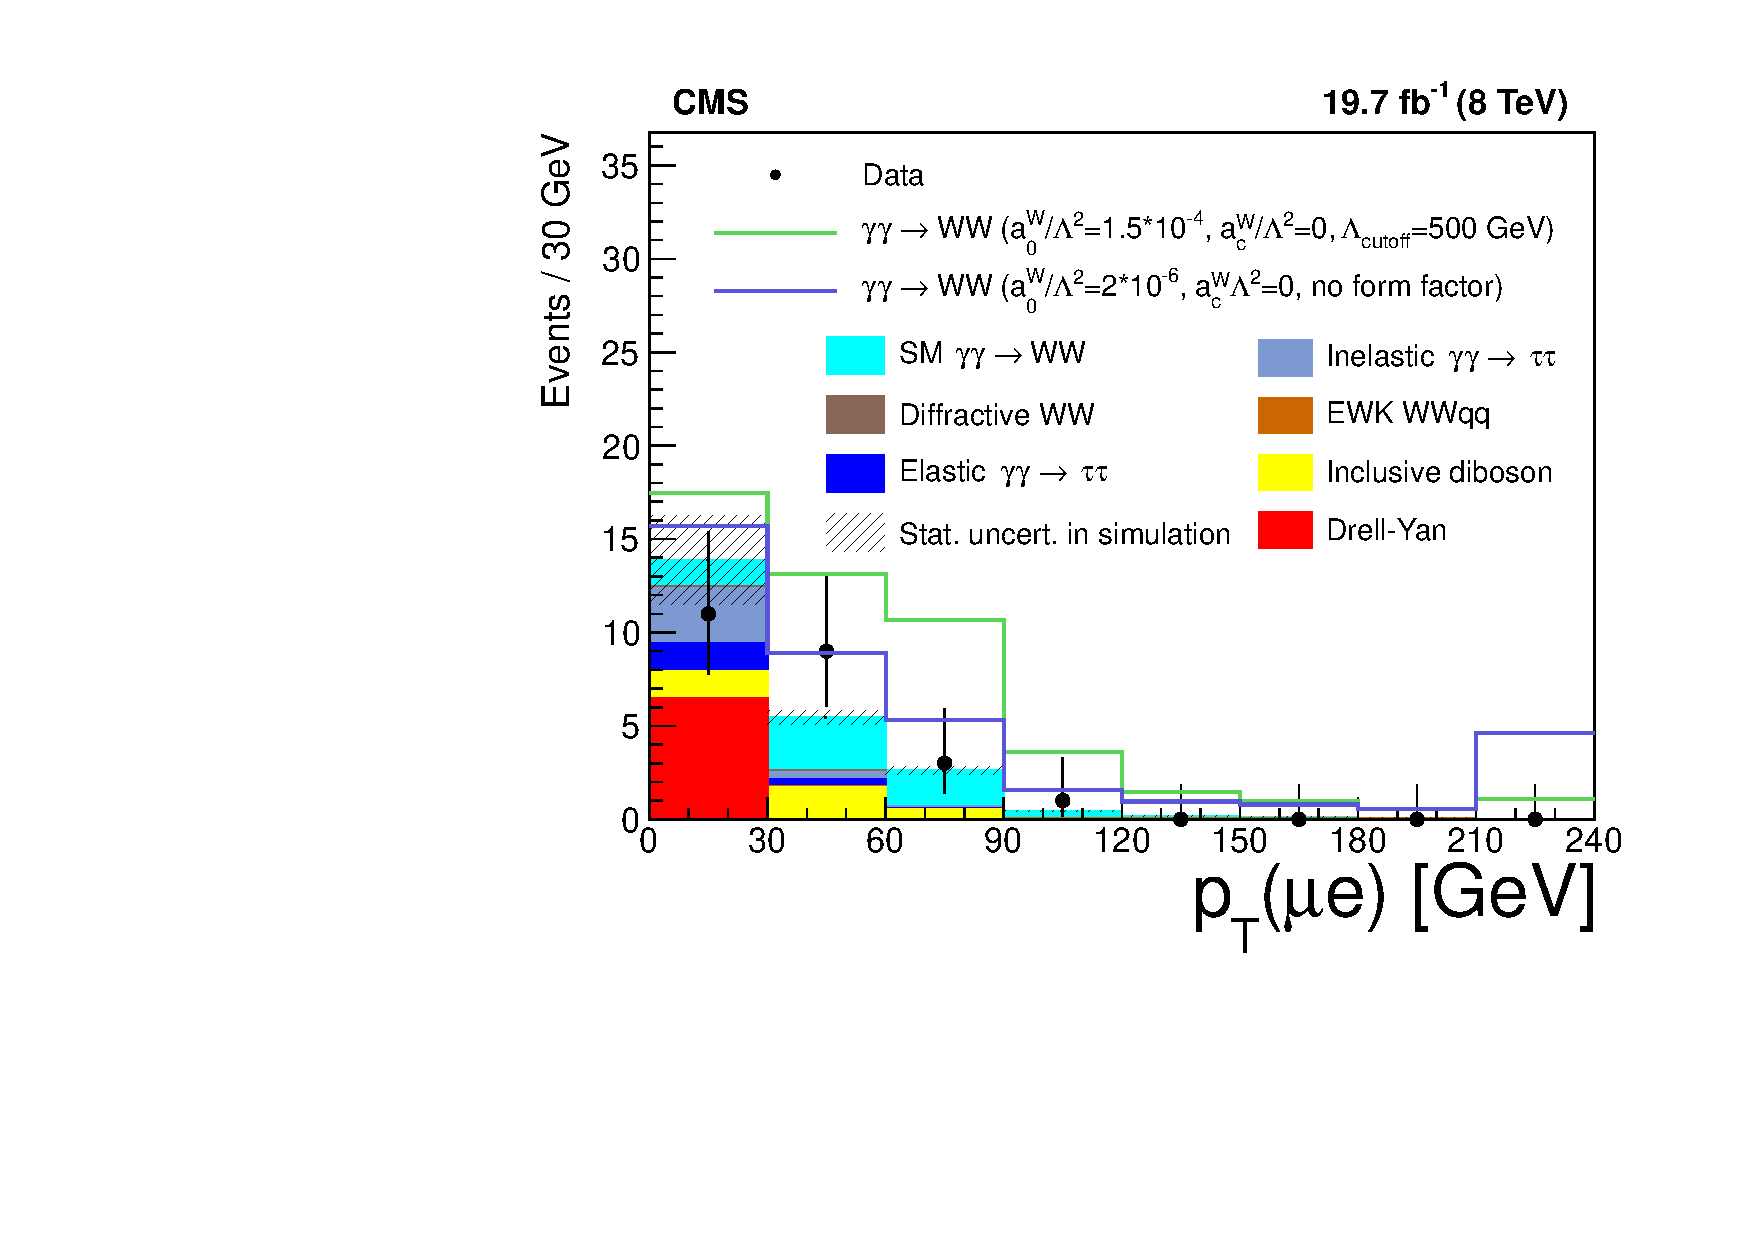
\includegraphics[width=.48\textwidth]{figures/ss-exclboson-ww-cms8tev-1.pdf}
%\includegraphics[width=.48\textwidth]{Figures/2016_01_29_UpdatedPlots/ee_tracks_
%pt30.pdf}
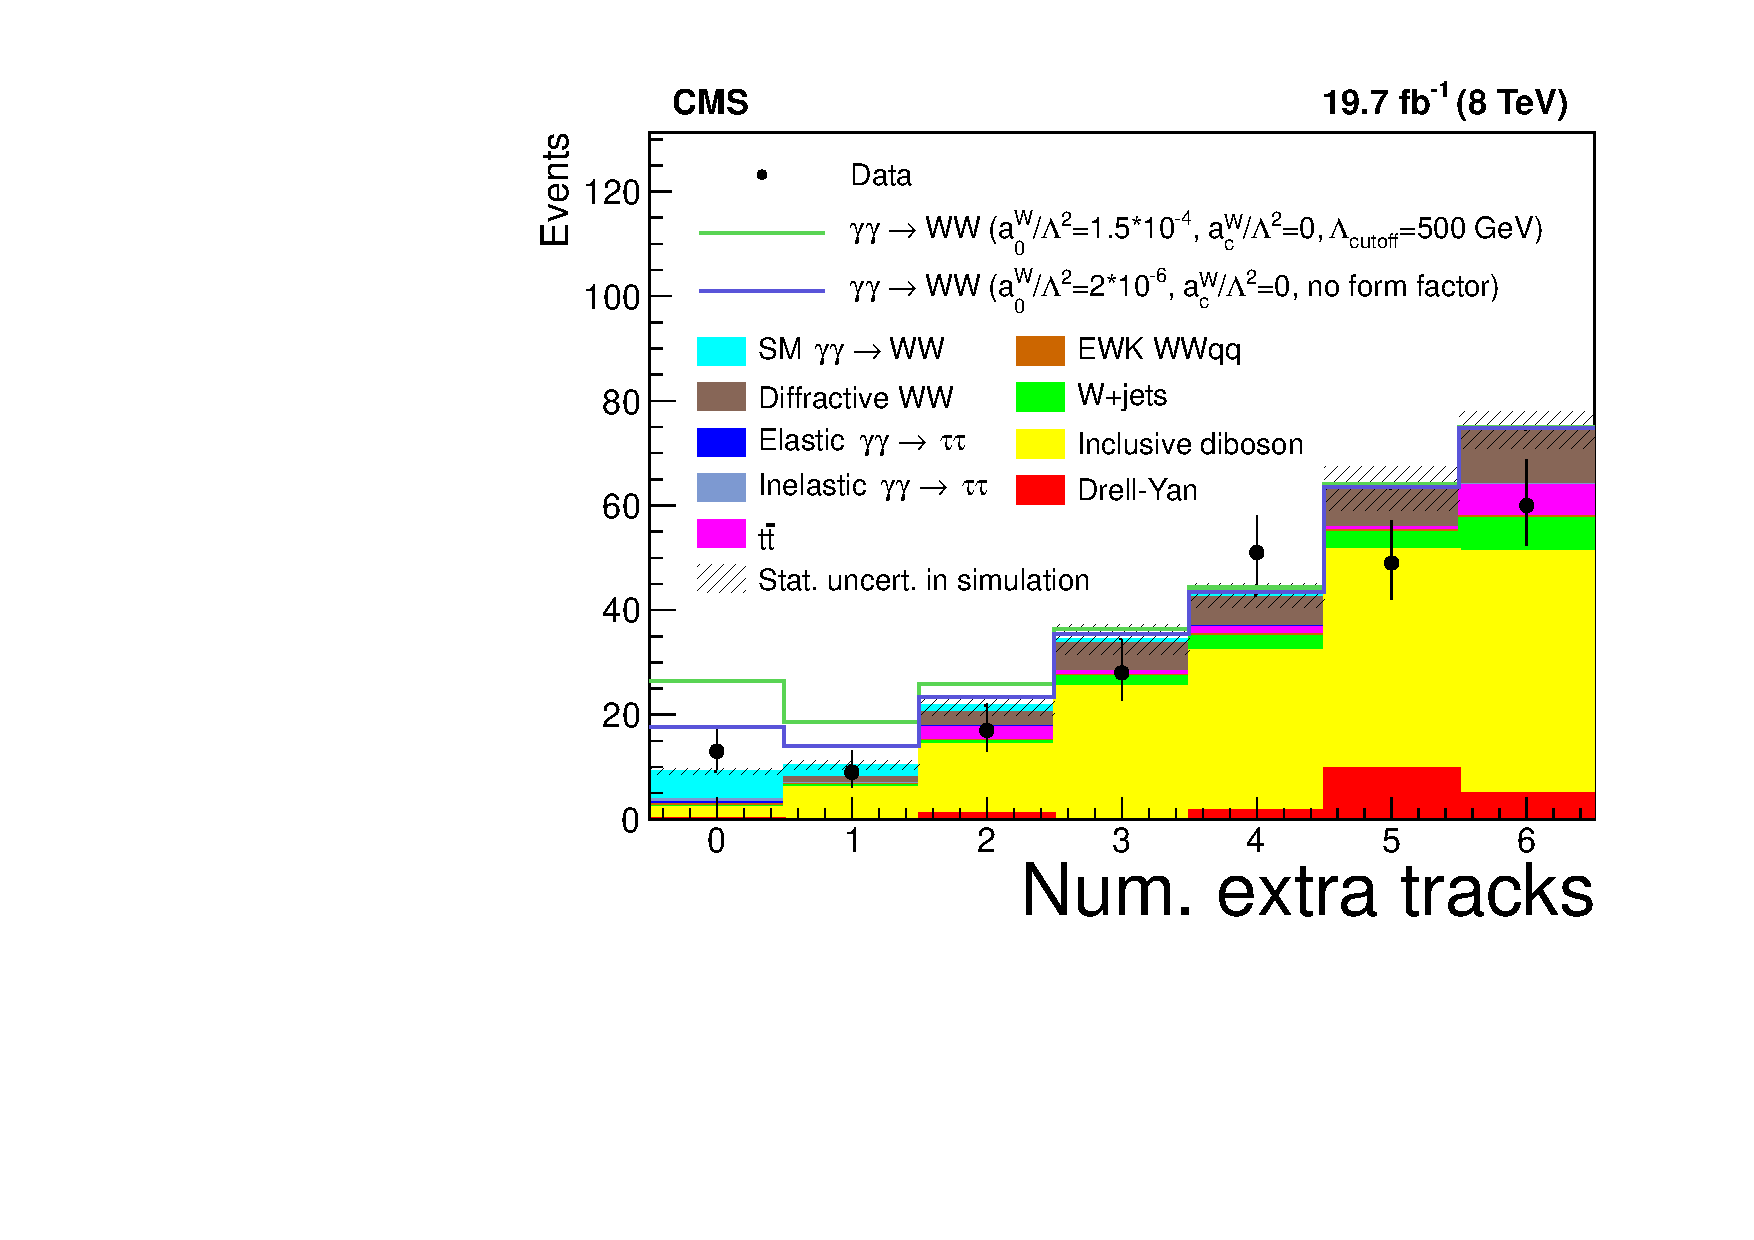
\includegraphics[width=.48\textwidth]{figures/ss-exclboson-ww-cms8tev-2.pdf}
\caption{Evidence for exclusive diboson production via $pp \to p^{(*)}W^+ W^- p^{(*)} \to p^{(*)}\mu^{\pm}e^{\mp}p^{(*)}$~\cite{Khachatryan:2016mud}.
Distributions of muon-electron transverse momentum for events with zero
 associated tracks (left), and extra-tracks multiplicity for events with $\pt(\mu^{\pm}e^{\mp}) > 30$ GeV (right).
 The data are shown by the points with error bars; the histograms indicate the expected SM signal and backgrounds.
\label{fig:ss-exclboson-ww-cms8tev}}
\end{figure}

The other exclusive diboson process for which the LHC has evidence is
same-sign WW production, via the process $qq \to WW +
2q \to \ell^\pm\ell^\pm + 2 \rm{jet} + \met$.  Similar to exclusive
single boson production, the final state of interest is a
superposition of several amplitudes at leading order, some of which
are purely electroweak and include triple and quartic gauge boson
interactions (see Fig.~\ref{fig:ss-exclboson-ww-sigdiagram}), and
some of which have the final state jets arise from QCD initial- and
final-state radiation. Through a suitable choice of final state phase
space, the electroweak amplitudes are enhanced and the associated
signal strength and distributions can be tested against the
electroweak theory.  The same-sign WW final state has the advantage
over other exclusive diboson channels ($W^+W^-$ or $WZ$) of a smaller
relative QCD amplitude and smaller multi-lepton backgrounds from top
quark, Drell-Yan, and WZ processes due to the same-sign dilepton
requirement.

An ATLAS analysis~\cite{Aad:2014zda} selects an ``inclusive region''
which is an admixture of electroweak and QCD contributions, and a VBS
signal region which is predominantly electroweak.  The inclusive
region requires two same-sign leptons with $\pt > 25$ GeV, $\met > 40$
GeV, and at least two jets with $m_{jj} > 500$ GeV for the two highest
$\pt$ jets; the VBS region further requires that the two highest $\pt$
jets are separated in rapidity, $|\Delta y_{jj}| > 2.4$.  To reduce
Drell-Yan background, events with dilepton mass less than 20 GeV or
dielectrons within 10 GeV of the Z mass are vetoed.  Top quark
background is reduced by vetoing events with b-tagged jets. Finally,
$WZ$ background is reduced by vetoing events with a third lepton with
muon $\pt > 6$ GeV or electron $\pt > 7$ GeV.  This results in 50
events selected for the inclusive region (as shown in
Fig.~\ref{fig:ss-exclboson-ww-ss}) and 34 for the VBS region.  About
half of selected events in either region are backgrounds from $WZ$,
$W\gamma$ with photon conversion, and misidentified leptons from jets
in $V$ + jet processes.  The significance of the signal in the
inclusive region is observed (expected) to be 4.5$\sigma$
(3.4$\sigma$), and for the VBS region the significance is observed
(expected) to be 3.6$\sigma$ (2.8$\sigma$).  The measured cross
sections in these two regions are $2.1\pm 0.5\rm{(stat)} \pm
0.3\rm{(syst)}$ fb and $1.3 \pm 0.4\rm{(stat)}\pm 0.2\rm{(syst)}$ fb,
comparing well with SM predictions
from \texttt{Powheg-Box}~\cite{Nason:2004rx,Frixione:2007vw,Alioli:2010xd,Jager:2009xx,Melia:2010bm,Melia:2011gk}
of $1.52 \pm 0.11$ fb and $0.95\pm 0.06$ fb, respectively.

The VBS cross section is used to constrain parameters of an effective
chiral Lagrangian theory of vector boson
scattering~\cite{Alboteanu:2008my}, calculated
by \texttt{Whizard}~\cite{Kilian:2007gr,Moretti:2001zz}: $−0.14
< \alpha_4 < 0.16$ and $−0.23 < \alpha_5 < 0.24$ limits are obtained
at 95\% CL.

A CMS analysis~\cite{Khachatryan:2014sta} selects events similar to
the ATLAS VBS region: two same-sign leptons with $\pt>20$ GeV, two
jets with $m_{jj}>500$ GeV and $|\Delta \eta_{jj}| > 2.5$, and $\met >
40$ GeV.  There is a same-flavor Drell-Yan veto for events with
dilepton mass less than 50 GeV or dielectrons within 15 GeV of the Z
mass, a veto of top-like events with secondary vertex or soft muon
tags, and a third lepton veto for $\pt > 10$ GeV.  The 12 events so
selected are shown in Fig.~\ref{fig:ss-exclboson-ww-ss}.  About half
of them are expected to be background, mostly from misidentified
leptons. The resulting excess has a significance of 1.9$\sigma$
(2.9$\sigma$) observed (expected) for the purely electroweak
amplitude.  The observed fiducial cross section is
$4.0^{+2.4}_{−2.0} \rm{(stat)} ^{+1.1}_{−1.0} \rm{(syst)}$ fb compared
to an expected cross section estimated from \texttt{VBFNLO}~\cite{Baglio:2014uba,Arnold:2011wj,Arnold:2008rz} of
$5.8 \pm 1.2$ fb.

The $m_{\ell\ell}$ distribution of selected events is used to obtain
95\% CL bounds on dimension 8 EFT couplings $f_{S,(0,1)}$,
$f_{M,(0,1,6,7)}$, and $f_{T,(0,1,2)}$~\cite{Eboli:2006wa}.  For
$f_{S,(0,1)}$, which can correspond to a spin-one VBS resonance, the
limits are $-42 \rm{TeV}^{-4} < f_{S,0}/\Lambda^4 < 43 \rm{TeV}^{-4}$
and $-129 \rm{TeV}^{-4} < f_{S,1}/\Lambda^4 < 131 \rm{TeV}^{-4}$.

\begin{figure*}[htb] {
\centering
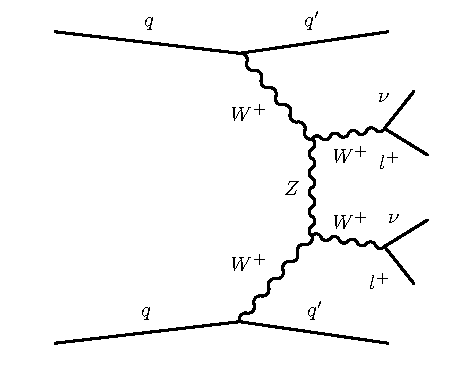
\includegraphics[width=0.315\textwidth]{figures/ss-exclboson-ww-diagram1.pdf}
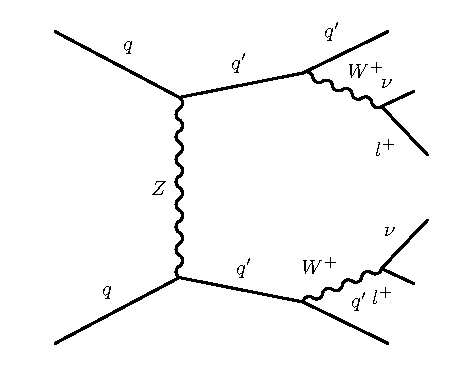
\includegraphics[width=0.35\textwidth]{figures/ss-exclboson-ww-diagram2.pdf}
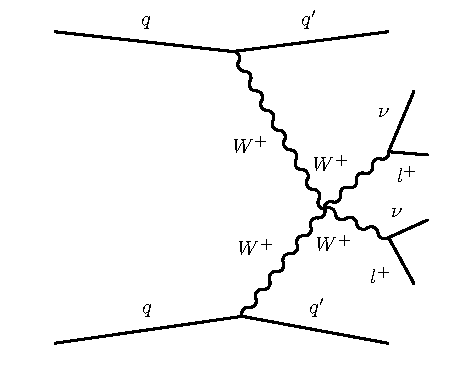
\includegraphics[width=0.315\textwidth]{figures/ss-exclboson-ww-diagram3.pdf}
\caption{
Representative Feynman diagrams for same-sign $WW$ production in association
with two jets from purely electroweak contributions:
(left) vector boson fusion,
(middle) bremsstrahlung-like,
and (right) multiperipheral production~\cite{Khachatryan:2014sta}.
\label{fig:ss-exclboson-ww-sigdiagram}}

}
\end{figure*}


\begin{figure}[p]
    \centering
    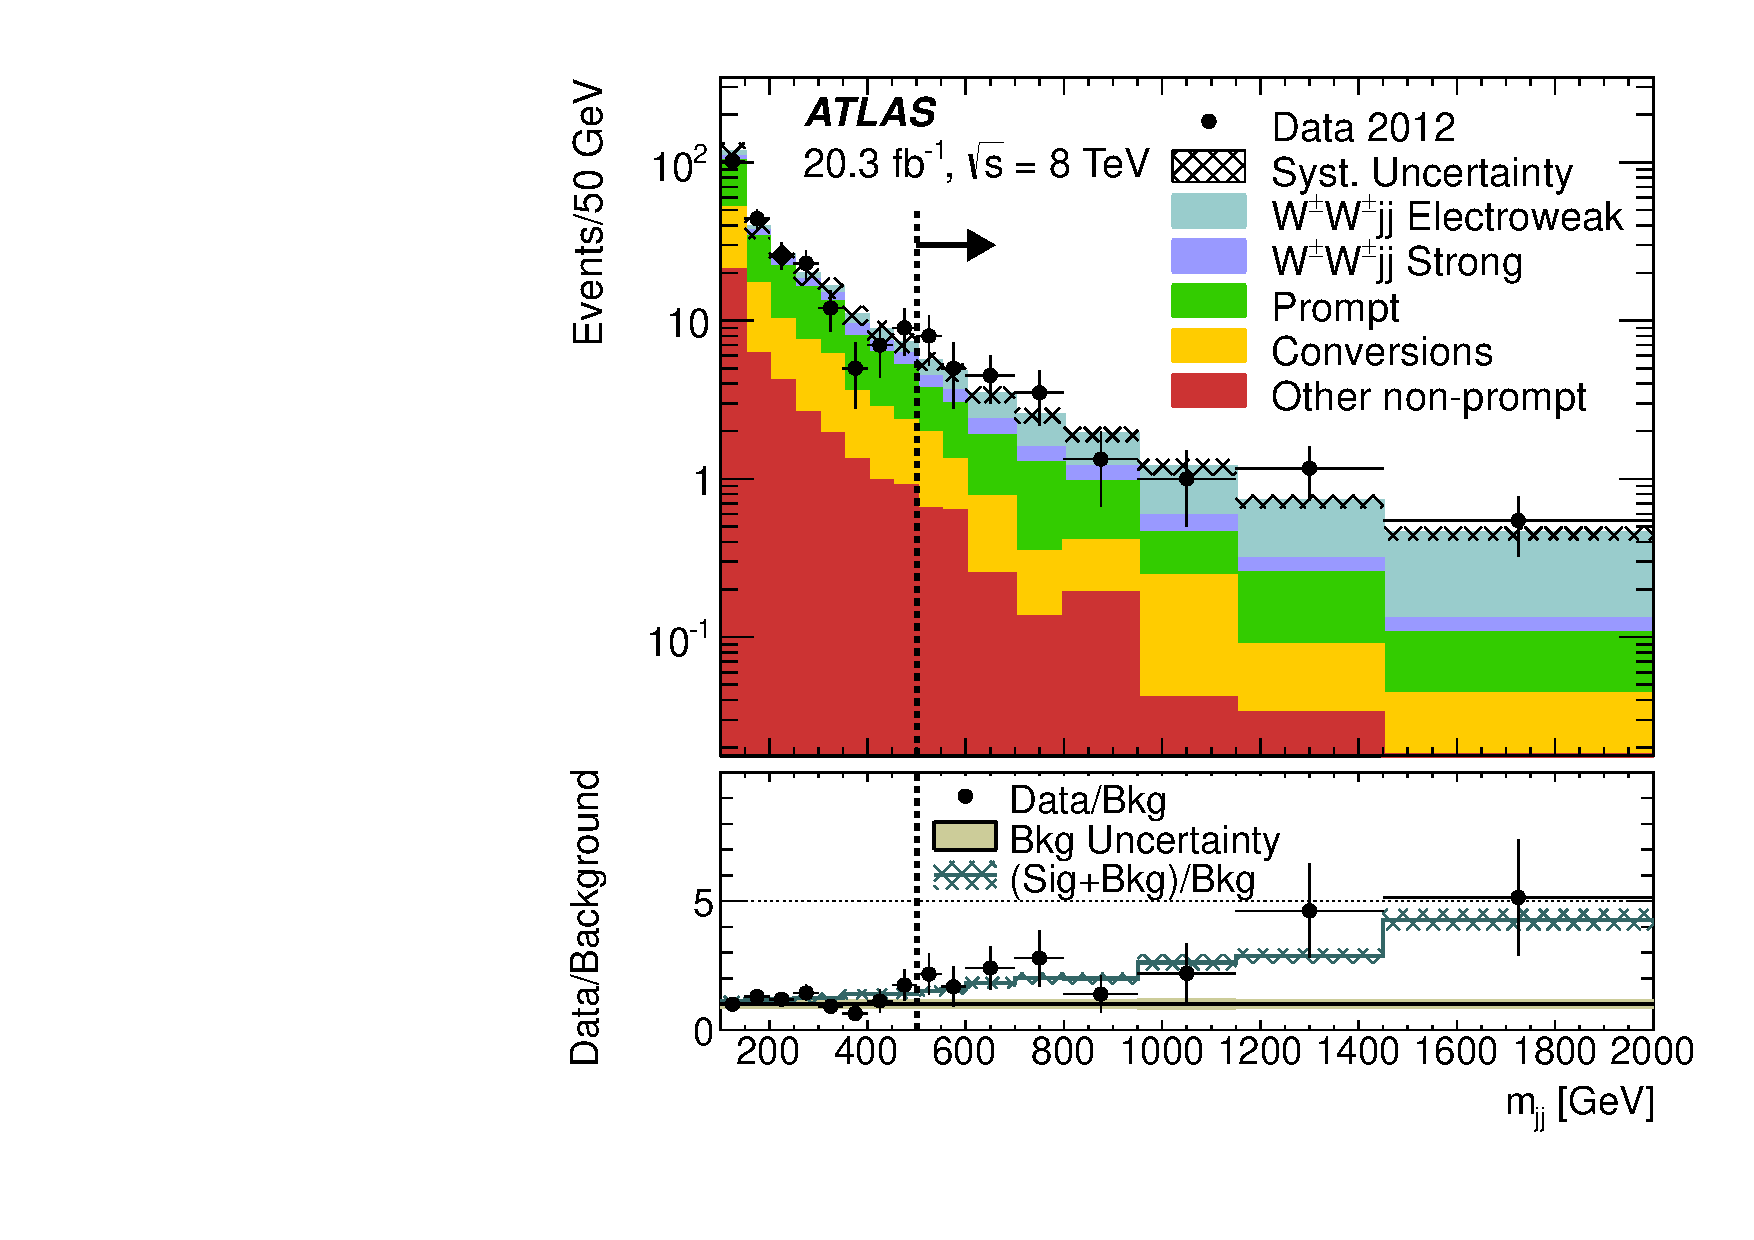
\includegraphics[width=0.45\textwidth]{figures/ss-exclboson-ww-ss-atlas8tev.pdf}
    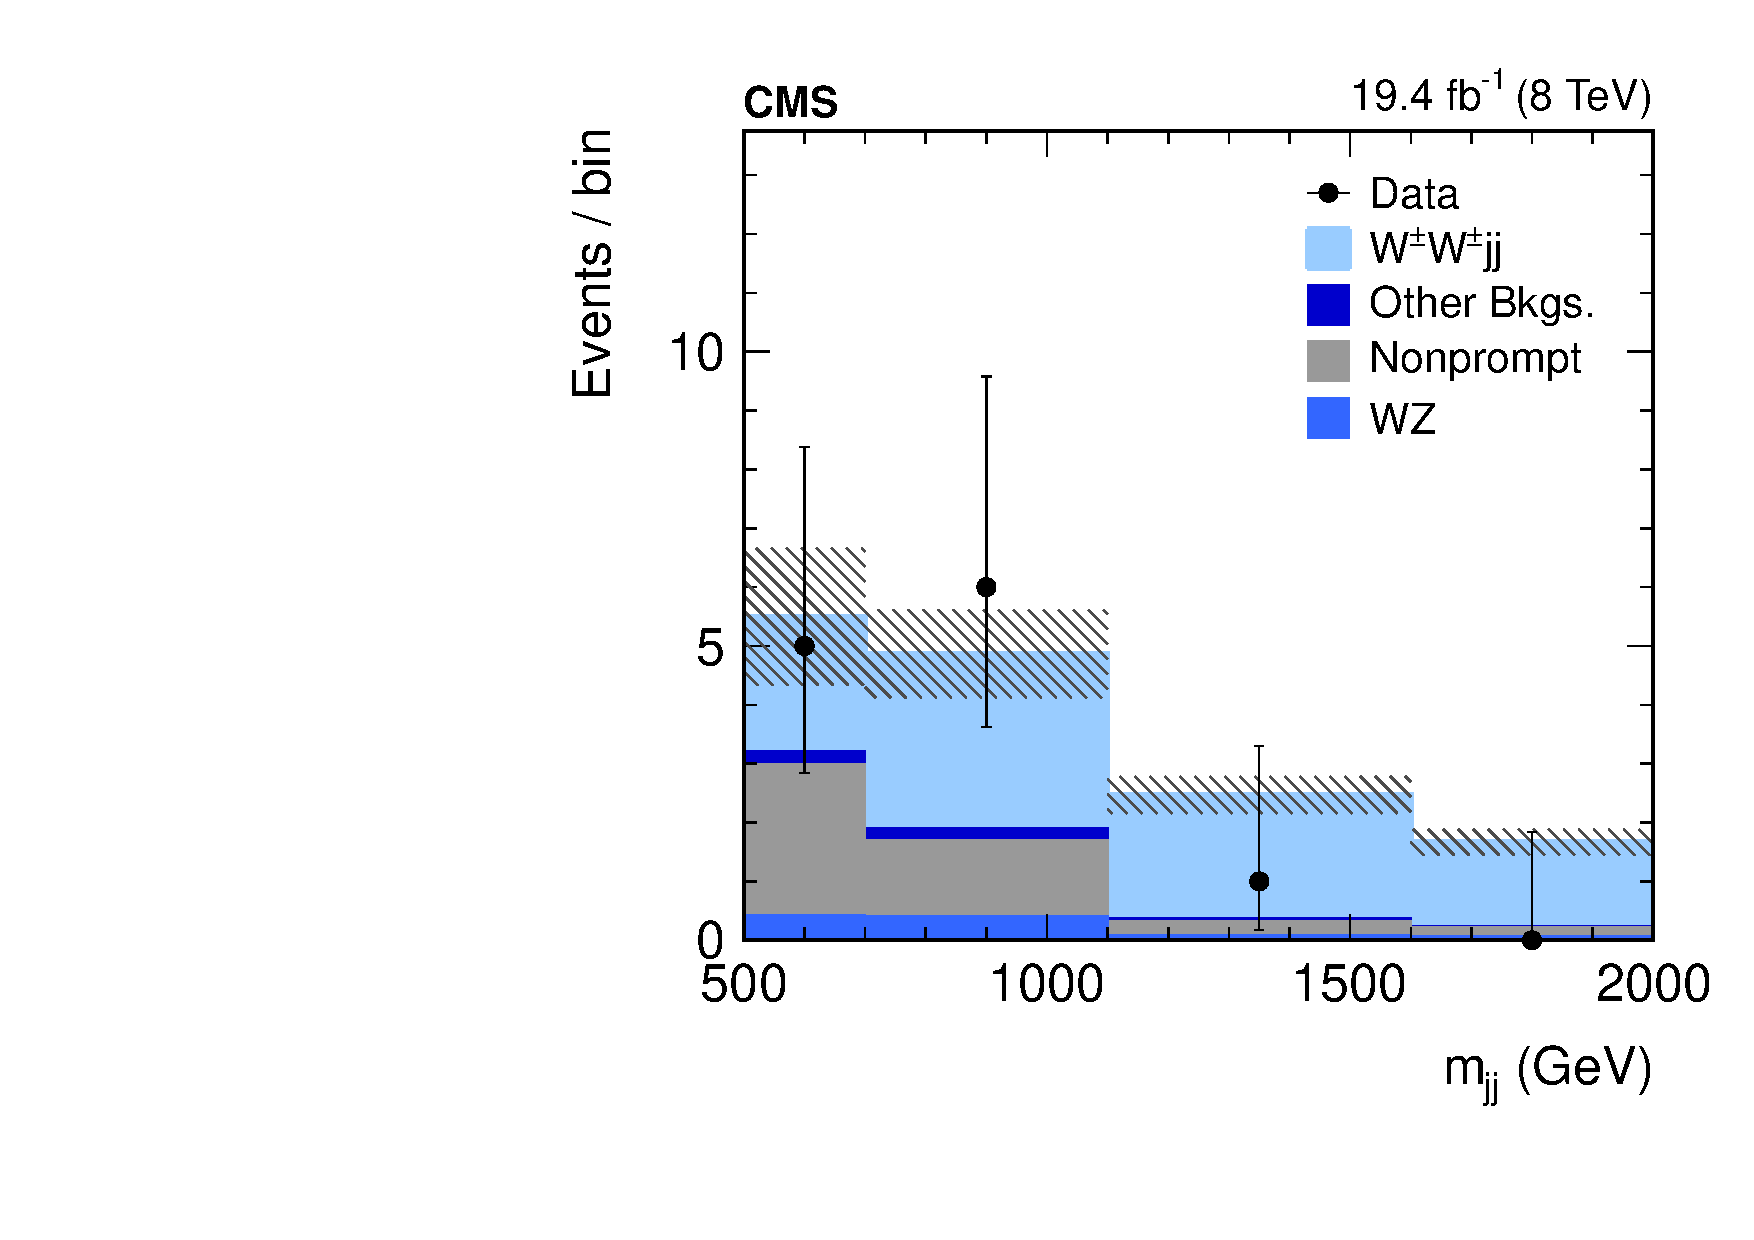
\includegraphics[width=0.45\textwidth]{figures/ss-exclboson-ww-ss-cms8tev.pdf}
    \caption{
    Left: Dijet invariant mass distribution of $W^{\pm} W^{\pm} jj$ candidates selected by ATLAS~\cite{Aad:2014zda}.  The inclusive signal region is indicated by the arrow.
    Right: Dijet invariant mass distribution of $W^{\pm} W^{\pm} jj$ candidates selected by CMS~\cite{Khachatryan:2014sta}.  }
    \label{fig:ss-exclboson-ww-ss}
\end{figure}
